\documentclass{IEEEcsmag}

\usepackage[colorlinks,urlcolor=blue,linkcolor=blue,citecolor=blue]{hyperref}
\expandafter\def\expandafter\UrlBreaks\expandafter{\UrlBreaks\do\/\do\*\do\-\do\~\do\'\do\"\do\-}
\usepackage{upmath,color}

\usepackage[spanish]{babel}
%\usepackage[latin1]{inputenc}
\usepackage[utf8]{inputenc}  

\jvol{1}
\jnum{1}
\paper{1}
\jmonth{Noviembre}
\jname{ITICs letters}
\jtitle{Proyectos Integradores}
\pubyear{2023}

\newtheorem{theorem}{Theorem}
\newtheorem{lemma}{Lemma}



\setcounter{secnumdepth}{0}

\begin{document}

\sptitle{Proyecto Integrador de Primer Semestre}

\title{Software de resolución de problemas de Ingeniería }

\author{Diego Antonio Badillo Morales, José Manuel Cortes Cerón, Oswaldo Gabriel Villaverde Mendoza, Carmen Anahi Cornejo Lopez, Sebastian Hernandez Angeles}
\affil{Instituto Tecnológico Superior del Occidente del Estado de Hidalgo, Mixquiahuala, Hgo., 42700, Mexico}

\markboth{ITSOEH/ITICS/PROYECTO INTEGRADOR PRIMER SEMESTRE}{THEME/FEATURE/DEPARTMENT}


\begin{abstract}
The project focuses on the resolution of 6 mathematical problems associated with the subjects of discrete mathematics and differential calculus of the first semester of the Information and Communication Technologies Engineering course. The objective of this project is to give a solution to each of the problems in an optimal way, using the knowledge of the subjects learned during the course. This file is available at \href{https://github.com/Joseecodm/ProyectoIntegrador.git}{https://github.com/Joseecodm/ProyectoIntegrador.git}.
\end{abstract}

\maketitle

\section{Introduccion}

\chapteri El manuscrito presenta la resolución de seis problemas matemáticos y lógicos propuestos en este proyecto de las asignaturas de Matemáticas discretas y calculo diferencial.
\newline
\newline
El objetivo principal de este proyecto es demostrar la comprensión de los conceptos y herramientas aprendidas durante ambas asignatura, aplicando de manera eficiente para dar solución a los problemas planteados, también se busca obtener la solución correcta así como justificar detalladamente cada paso del proceso seguido, para conseguir estos objetivos se usó la metodología de las 6D la cual consiste en descripción de problema, definición de la solución, diseño de la solución, desarrollo de la solución, depuración y pruebas, documentación, como resultado, se lograron resolver los problemas de la manera mas optima, demostrando con ello la comprensión de conceptos clave tan relevantes para el desempeño académico y profesional como ingenieros en tecnologías de la información y la comunicación



\section{Problema 1}
\begin{enumerate}
    
\item  Descripción del problema

El problema consiste en calcular la ecuación de una recta y su ángulo con el eje horizontal, dados dos puntos de la recta.\newline

\item  Definición del problema:

Los datos del problema son los siguientes:

Los valores de las coordenadas x1 y y1 de uno de los puntos de la recta.
 
Los valores de las coordenadas x2 y y2 del 
otro punto de la recta.

El deseo del problema es obtener los siguientes resultados:

La ecuación de la recta, en la forma y = m*x + b.
 
El ángulo con el eje horizontal, en grados.\newline

\item  Diseño de la solución:


De acuerdo a la Figura ~\ref{fig:diagramaP1}


La solución se puede dividir en los siguientes pasos:

 - Calcular la pendiente de la recta, m.

 -Calcular el ángulo de la recta, a, utilizando la fórmula a = atan(m).

 -Convertir el ángulo a grados, a Grados = a * 180 / PI.

-Obtener la ecuación de la recta, y = m * x + b, donde b = y1 - m * x1.\newline

\begin{figure}
\caption{Diagrama de flujo problema uno}
\centerline{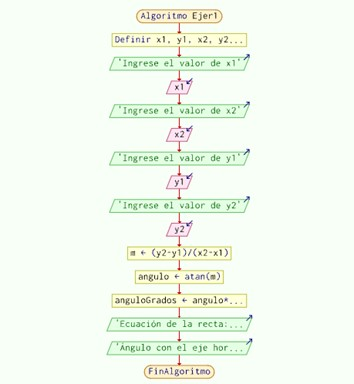
\includegraphics[width=0.5\textwidth]{./latex-imagenes/diagramaProb1.jpg}}
\vspace*{7pt}
\label{fig:diagramaP1}
\end{figure}

\item  Desarrollo de la solución:



	El código comienza con las importaciones necesarias y algunos comentarios que proporcionan información sobre la clase (figura ~\ref{fig:codigoP1}). 
 
\begin{figure}
\caption{Codigo Problema Uno}
\centerline{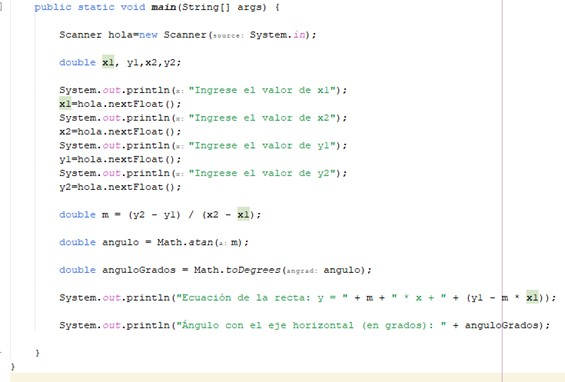
\includegraphics[width=0.5\textwidth]{./latex-imagenes/codigoprob1.jpg}}
\vspace*{7pt}
\label{fig:codigoP1}
\end{figure}

	La función main comienza solicitando al usuario las coordenadas de A y B.
 
	Después para la ecuación de la recta para (y) se utiliza la formula 
 
 \begin{equation}
     (y2 - y1) / (x2 - x1)
 \end{equation}
 y se almacena en la variable m.
 
	Después para (x) se utiliza la siguiente operación 
  \begin{equation}
      (y1 - m * x1)
  \end{equation}
	Y para sacar el ángulo en grados se utiliza la función Math.atan(m) para calcular el ángulo en radianes y después se usa Math.toDegrees() para pasar de radianes a grados.\newline
	Y finaliza dándote el resultado de la Ecuación de la recta y el Ángulo con el eje horizontal.\newline
\item  Depuración y pruebas \newline
	Prueba basica:\newline
	(x1, y1) = (0, 0)\newline
	(x2, y2) = (1, 1)\newline

	Ingrese el valor de x1

	Ingrese el valor de x2

	Ingrese el valor de y1

	Ingrese el valor de y2\newline

Ecuación de la recta: y = 1.0  x = 0.0
Angulo con el eje horizontal (en grados):  45.0

\end{enumerate}
\vspace*{5pt}






\section{Problema 2}
\setlength{\parskip}{5pt}
\begin{enumerate}
\item Descripción del problema:
Dada la ecuación que ingrese se regresara los valores de las raíces en caso de que estén sobre el conjunto de los números reales, en el caso de que no indicara la solución esta en el conjunto de los números complejos.\newline

\item Definición del problema:
	
 Se solicita al usuario que ingrese a, b y c.
	
 Se calcula el discriminante de la ecuación cuadrática, dado por la formula b2-4ac.
	
 Te arrojará como resultado: los valores de (x1, x2) y escribirá si las raíces son reales, idéntica o si no tiene.\newline

 \item Diseño de la solución:
  
\begin{figure}
\caption{Diagrama Problema Dos}
\centerline{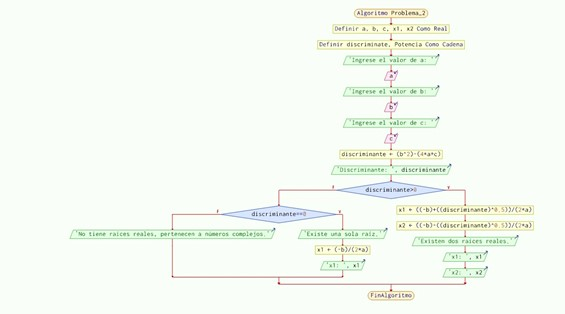
\includegraphics[width=0.5\textwidth]{./latex-imagenes/diagramaProb2.jpg}}
\vspace*{7pt}
\label{fig:diagramaP2}
\end{figure}

 La solución del problema se basa en los siguientes pasos (figura ~\ref{fig:diagramaP2}):
1.	Ingresar los datos de a, b y c.
2.	Modificar los datos de la ecuación.
3.	Dado el resultado se darán dos respuestas que serán x1 y x2.
4.	Y te arrojara un mensaje que siga si hay dos raíces, solo una o ninguna.\newline

\item Desarrollo de la solución:

\begin{figure}
\caption{Codigo Problema Dos}
\centerline{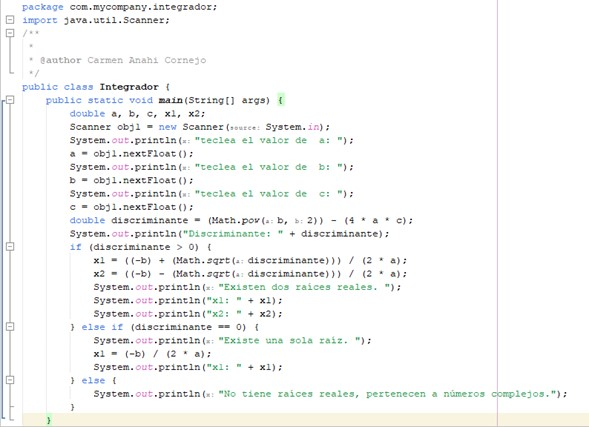
\includegraphics[width=0.5\textwidth]{./latex-imagenes/codigoprob2.jpg}}
\vspace*{7pt}
\label{fig:codigoP2}
\end{figure}

Antes que nada, tenemos que tener claro que la ecuación cuadrática siempre será (figura ~\ref{fig:codigoP2}):

 \begin{equation}
〖ax〗^2+bx+c=0
\label{eq:recta}
\end{equation} 
siempre que la ecuación esta ordenada podemos ver cuál es el valor de a, b y c.
	
 El código comienza import Scanner y algunos comentarios que nos proporcionan información sobre la clase.
	
 Definimos a, b, c, x1, x2 como double para que pueda ver resultados decimales.
	
 Se crea un objeto como Scanner para poder leer a, b y c. 
	
 Al ya tener ingresado los valores de a, b y c los remplazaremos en la ecuación 
 
  \begin{equation}
(-b+-	√(b²-4ac))/(2a)
\label{eq:rectaa}
\end{equation} 
 que es de tipo double.
	
 Para la siguiente parte tuvimos que tener claro que:
 
-Si el discriminante > cero, hay dos raíces reales distintas.

-Si el discriminante = cero, existe una sola raíz real idéntica. 

-Si el discriminante < cero, no tiene raíces reales, pertenecen a números complejos.

Después de eso utilice un if  (discriminante > 0) para poder sacar los dos resultados los cuales son x1 que es positivo y x2 que es negativo.


Seguido con un else if (disciminante==0) que ejecutara la ecuación:         
\begin{equation}
  x1= (-b) / ( 2 * a )  
\end{equation}


Finalizamos con un else que solo ejecutara un texto diciendo “No tiene raíces reales, pertenece a números completos”\newline
\item Depurar:

\begin{figure}
\caption{Prueba de escritorio Problema Dos}
\centerline{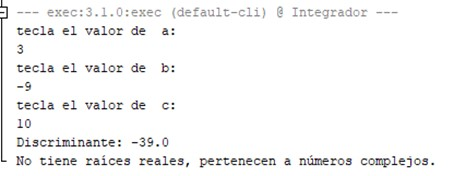
\includegraphics[width=0.5\textwidth]{./latex-imagenes/pruebaDeskEj2.jpg}}
\vspace*{7pt}
\label{fig:pruebaP2}
\end{figure}

Se comprobó si el código se ejecuta correctamente y para eso se realizó pruebas de escritorio(figura ~\ref{fig:pruebaP2}).

\end{enumerate}
\vspace*{5pt}

\section{Problema 3}
\begin{enumerate}

\item Descripción del problema:
•	Problema: Dada una circunferencia con centro en el punto C con coordenadas (X1, X2) y el radio R, evaluar si un punto T con coordenadas (X2, Y2) está dentro del área de la circunferencia.

\item Definición del problema:
Problema: Saber si un punto se encuentra dentro o fuera de un circulo.

Entradas: El punto que se desea encontrar.

Salidas: Saber si el punto se encuentra dentro o fuera de circulo 

\item Diseñar de solución (figura ~\ref{fig:diagramaP3}):
\begin{figure}
\caption{Diagrama Problema Tres}
\centerline{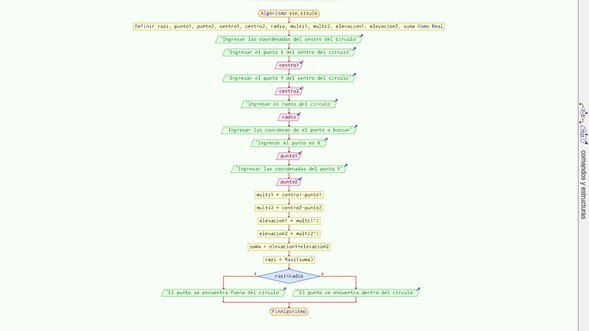
\includegraphics[width=0.5\textwidth]{./latex-imagenes/diagramaProb3.jpg}}
\vspace*{7pt}
\label{fig:diagramaP3}
\end{figure}

\item Desarrollar  (figura ~\ref{fig:codigoP3}):

\begin{figure}
\caption{Codigo Problema Tres}
\centerline{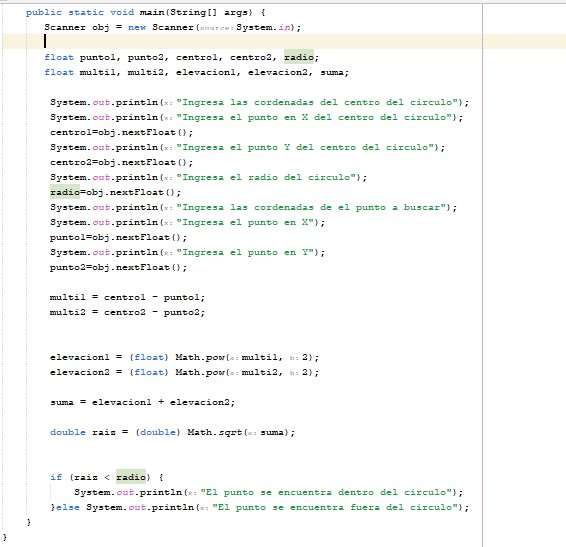
\includegraphics[width=0.5\textwidth]{./latex-imagenes/codigoprob3.jpg}}
\vspace*{7pt}
\label{fig:codigoP3}
\end{figure}
Se crean dos objetos Scanner (x1, x2) para leer la entrada del usuario. 

Se solicita que ingrese el radio del círculo.

Se crea un objeto Scanner (r) para leer la entrada del usuario. 

Se solicita que ingrese las coordenadas del punto a buscar.

Se crea dos objetos Scanner (x2, y2) para leer la entrada del usuario.

Se realiza una operación matemática en donde se restan las coordenadas y se elevan al cuadrado, después se suman ambos resultados y sacas raíz cuadrado.

Usamos un if para saber si el punto esta fuera o dentro del círculo, si la distancia es menor al radio el punto se encontrara dentro del círculo, de lo contrario el punto se encontraría fuera del círculo.

\item Depurar (figura ~\ref{fig:pruebaP3}):

\begin{figure}
\caption{Prueba de escritorio Problema Tres}
\centerline{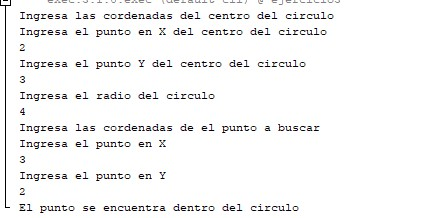
\includegraphics[width=0.5\textwidth]{./latex-imagenes/pruebaDeskEj3.jpg}}
\vspace*{7pt}
\label{fig:pruebaP3}
\end{figure}

 Se comprobó si el código se ejecuta correctamente y para eso se realizó pruebas de escritorio.
 
\end{enumerate}

\vspace*{5pt}
\section{Problema 4}
\begin{enumerate}

\item  Descripción del problema
El problema resuelto con este código es la conversión de un número decimal entero a binario. El número binario se representa como una cadena de bits, donde cada bit tiene un valor de 0 o 1.\newline

\item  Definición del problema


 El tipo de datos del número decimal. En este caso, el número decimal es un número entero.

 El rango de valores del número decimal. En este caso, el número decimal puede tomar cualquier valor entero, desde -2 elevado a 32 hasta 2 elevado a 32 - 1.

 El formato del número binario. En este caso, el número binario se representa como una cadena de bits, donde cada bit tiene un valor de 0 o 1.\newline


\item  Diseño de la solución
(figura ~\ref{fig:diagramaP4}):

\begin{figure}
\caption{Diagrama de flujo Problema Cuatro}
\centerline{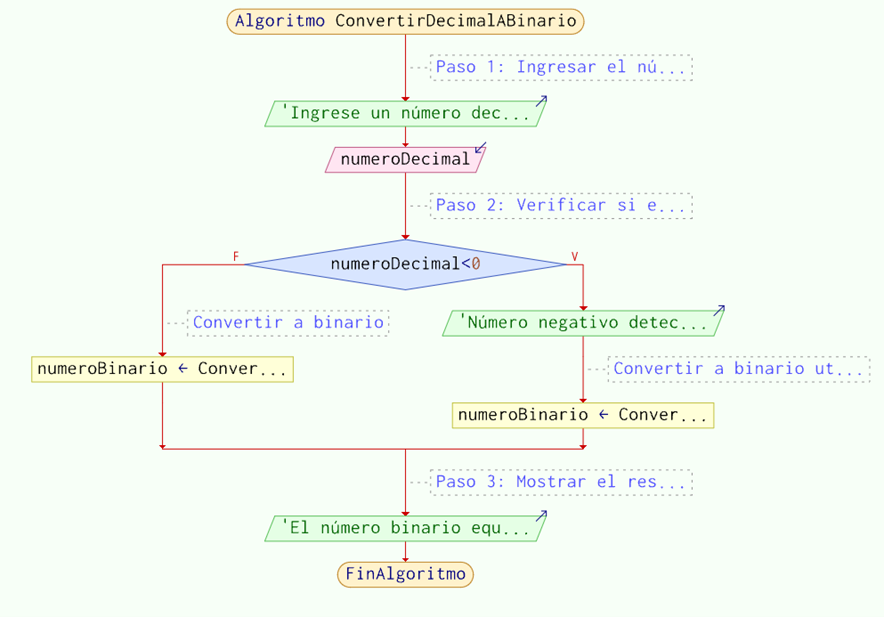
\includegraphics[width=0.5\textwidth]{./latex-imagenes/diagramaprob4.png}}
\vspace*{7pt}
\label{fig:diagramaP4}
\end{figure}
La solución al problema se basa en los siguientes pasos:
1.	Comprobar si el número es positivo o negativo.
2.	Convertir el número decimal a binario.
3.	Si el número es negativo, aplicar el método de complemento a2.\newline







\item  Desarrollo de la solución(figura ~\ref{fig:codigoP4}):

1. Comprobar si el número es positivo o negativo.

Este paso es sencillo. Se puede utilizar el operador de comparación >= para comprobar si el número es mayor o igual que cero.

2. Convertir el número decimal a binario, si es positivo o negativo.
Si el número es positivo, se puede utilizar el método toBinaryString() de la clase Integer para convertir el número decimal a binario.

Si el número es negativo, se aplica el método de complemento a2.

El método de complemento a2 consiste en los siguientes pasos:
 
 Invertir el orden de los bits del binario del número negativo.
 Añadir un 1 al principio.\newline
 
Ejemplo:
El número decimal -1 se convierte a binario en 11111111111111111111111111111110 (en complemento a2).\newline


\begin{figure}
\caption{Codigo Problema Cuatro}
\centerline{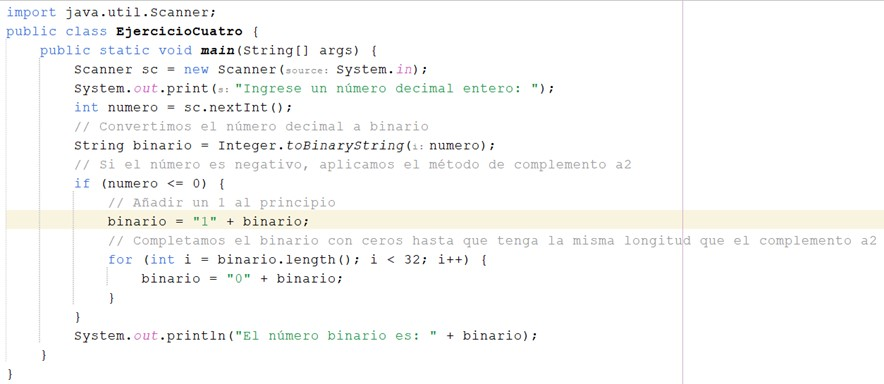
\includegraphics[width=0.5\textwidth]{./latex-imagenes/codigoprob4.jpg}}
\vspace*{7pt}
\label{fig:codigoP4}
\end{figure}
 



\item  Depuración y pruebas

Número decimal: 10

Número binario: 1010

Número decimal: -1

Número binario : 

11111111111111111111111111111110

Número decimal: 0

Número binario: 0

    
\end{enumerate}
\vspace*{5pt}


%Jose%
\section{Problema 5}
\setlength{\parskip}{5pt}
\begin{enumerate}
\setlength{\parskip}{5pt}
\item Descripción del problema:

Dado un numero binario de n bits regresar su equivalente en decimal.


\item Definición del problema:

• Problema: Convertir un número binario ingresado por el usuario a su equivalente decimal. 

• Entradas: El número binario ingresado por el usuario. 

• Salidas: El equivalente decimal del número binario.

\item Diseño de solución:

(figura ~\ref{fig:diagramaP5})

Solicitar al usuario un número binario.
Verificar si el número es binario (contiene solo 0 y 1).
Si no es binario, solicitar nuevamente el número binario.
Convertir el número binario ingresado a su equivalente decimal.
Mostrar el equivalente decimal del número binario.

\begin{figure}
\caption{Diagrama de flujo Problema Cinco}
\centerline{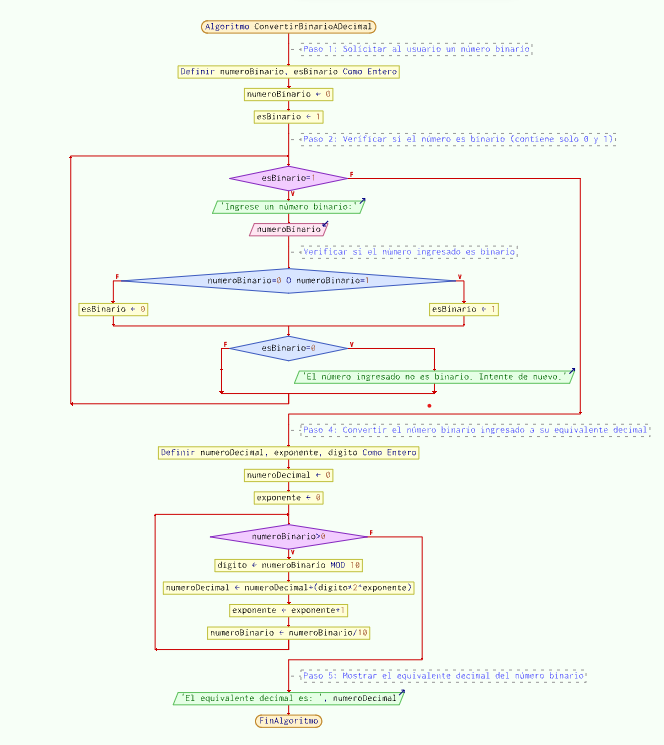
\includegraphics[width=0.5\textwidth]{./latex-imagenes/diagramaprob5.png}}
\vspace*{7pt}
\label{fig:diagramaP5}
\end{figure}

\setlength{\parskip}{5pt}   

\item Desarrollar (figura ~\ref{fig:codigoP5}):

El código comienza con las importaciones necesarias y algunos comentarios que proporcionan información sobre la clase.

Función 'main': 

• La función main comienza declarando una variable numeroBin para almacenar el número binario ingresado por el usuario. 

• Se crea un objeto Scanner (binario) para leer la entrada del usuario. 

• Se usa un bucle do-while para pedir al usuario que ingrese un número binario. Continúa solicitando la entrada hasta que se ingrese un número binario válido (solo 0 y 1). 

• Después de obtener un número binario válido, llama a la función binarioADecimal para convertirlo a su equivalente decimal y muestra el resultado.


Función 'esBinario':

Esta función toma un String como argumento y verifica si el número ingresado consiste solo en caracteres '0' y '1'. Retorna true si es un número binario válido; de lo contrario, retorna false.

Función 'binarioADecimal':

• Esta función convierte un número binario dado en un número decimal. 

• Itera sobre cada dígito del número binario, convirtiendo cada dígito a su equivalente decimal y sumándolo al resultado final. 

• Usa la fórmula de conversión de binario a decimal:
\begin{equation}
    suma de (dígito * 2 $^{posicion}$)
\end{equation}
, donde la posición comienza desde 0 y se incrementa hacia la izquierda en el número binario.
\begin{figure}
\caption{Codigo Problema Cinco}
\centerline{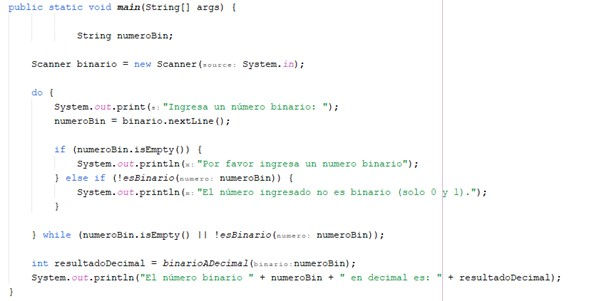
\includegraphics[width=0.5\textwidth]{./latex-imagenes/codigoprob5.png}}
\vspace*{7pt}
\label{fig:codigoP5}
\end{figure}

\item Depurar:

• Verifiqué si hay errores, comprobé si el código se ejecuta correctamente y realicé pruebas de escritorio para asegurarme de que la conversión binario-decimal funcionara correctamente.\newline

\end{enumerate}

\section{Problema 6}

\begin{enumerate}


\item Definición del problema:\newline

Se busca obtener una expresión booleana que represente de manera fidedigna las salidas de una tabla de verdad de n bits.\newline\newline
 \item  Diseño:\newline
•	Entrada de datos:
Se requiere la tabla de verdad de n bits que contiene las combinaciones de entrada y sus salidas correspondientes.
•	Análisis de datos:
Identifique las combinaciones de entrada que producen una salida de 1 y se utiliza esta información para construir la expresión booleana.\newline
Algoritmo:

1.	Inicio

2.	Ingresar la cantidad de bits (numBits):

•	Se lee la cantidad de bits que se utilizarán en la tabla de verdad.

3.	Inicializar el arreglo de letras (letras):

•	Se define un conjunto de letras (A, B, C, D) para representar los bits.

4.	Calcular el total de combinaciones posibles (totalCombinaciones):

•	Se calcula el número total de combinaciones posibles de bits usando la fórmula 
\begin{equation}
    2^n^u^m^B^i^t^s
\end{equation}

5.	Mostrar la tabla de verdad:

•	Se muestran las letras que representan los bits y se crea la estructura de la tabla.

6.	Generar expresiones booleanas para las filas con valor de salida 1:

•	Para cada combinación de bits posible:

•	Se recorren los bits y se genera la expresión booleana correspondiente.

•	Si el bit es 0, se muestra la negación de la letra; si es 1, se muestra la letra sola.




\item Desarrollo:

•	Identificar combinaciones con salida 1: Se revisan todas las combinaciones de la tabla de verdad y se registran aquellas que tengan una salida de 1.

•	Crear la expresión booleana: Se utilizan las combinaciones identificadas con salida 1 para generar la expresión booleana .

Configuración inicial y solicitud de datos(figura ~\ref{fig:codigo1P6}):

\begin{figure}
\caption{Codigo Uno Problema Seis}
\centerline{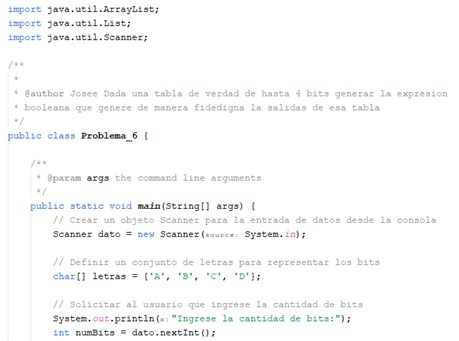
\includegraphics[width=0.5\textwidth]{./latex-imagenes/codigo1prob6.jpg}}
\vspace*{7pt}
\label{fig:codigo1P6}
\end{figure} 


•	Importa las clases necesarias (Scanner, ArrayList, List).
•	Define un conjunto de letras para representar los bits.
•	Crea un objeto Scanner para la entrada de datos.
•	Pide al usuario que ingrese la cantidad de bits.

Generación de la tabla de verdad y solicitud de valores de salida(figura ~\ref{fig:codigo2P6}):
\begin{figure}
\caption{Codigo Dos Problema Seis}
\centerline{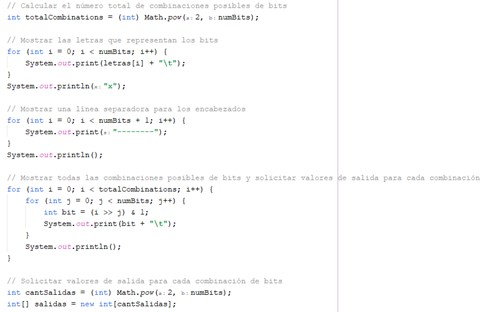
\includegraphics[width=0.5\textwidth]{./latex-imagenes/codigo2prob6.jpg}}
\vspace*{7pt}
\label{fig:codigo2P6}
\end{figure}


•	Calcula el número total de combinaciones posibles de bits.

•	Muestra las letras que representan los bits y una línea separadora.

•	Muestra todas las combinaciones posibles de bits.

•	Solicita valores de salida para cada combinación de bits.

Procesamiento de valores de salida y generación de expresiones booleanas (figura ~\ref{fig:codigo3P6}):
\begin{figure}
\caption{Codigo Tres Problema Seis}
\centerline{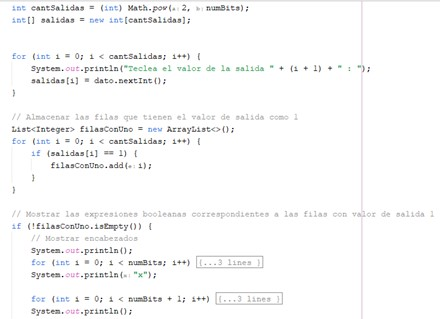
\includegraphics[width=0.5\textwidth]{./latex-imagenes/codigo3prob6.jpg}}
\vspace*{7pt}
\label{fig:codigo3P6}
\end{figure}

•	Solicita valores de salida para cada combinación de bits.

•	Almacena en una lista las filas que tienen un valor de salida igual a 1.

•	Si hay filas con valor de salida 1, se procede a mostrar las expresiones booleanas correspondientes a estas filas.
En caso contrario, muestra un mensaje indicando que no hay filas con valor 1.


Generación de expresiones booleanas para filas con valor de salida 1(figura ~\ref{fig:codigo4P6}):
\begin{figure}
\caption{Codigo Cuatro Problema Seis}
\centerline{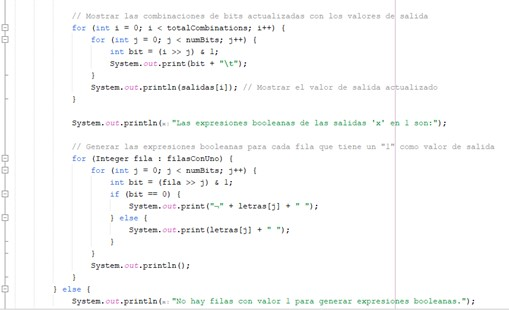
\includegraphics[width=0.5\textwidth]{./latex-imagenes/codigo4prob6.jpg}}
\vspace*{7pt}
\label{fig:codigoeP6}
\end{figure}
 
Explicación:

•	Si hay filas con valor de salida igual a 1, muestra los encabezados y las combinaciones de bits con sus valores de salida.

•	Genera las expresiones booleanas correspondientes a las filas que tienen un valor de salida igual a 1. Las expresiones se construyen usando las letras que representan los bits y, si es necesario, la negación de estas letras.\newline\newline

\item Depuración:

•	Verificación de la lógica: Se revisa que la expresión generada por la tabla de verdad produzca los resultados esperados.

•	Manejo de errores: Se valida que la expresión generada sea coherente y represente correctamente la tabla de verdad.\newline\newline

 \item Pruebas:
•	Validación de la expresión: Se prueba la expresión generada utilizando la tabla de verdad original para confirmar que reproduce los resultados correctamente.

\end{enumerate}

\section{Agradecimientos}

Cada idea, cada contribución y cada hora de trabajo dedicada ha desempeñado un papel fundamental en el éxito de este proyecto. Vuestra dedicación y compromiso han sido pilares esenciales para alcanzar nuestros objetivos. Reconozco y valoro profundamente el arduo trabajo y la colaboración ejemplar que cada uno de nosotros demostrado.

\section{Referencias}

%Carmen 
Carmen Anahi Cornejo López es una estudiante del ITSOEH, en el cual cursa su primer año en la carrera de Tic´s , nacida en Mixquiahuala de Juárez hidalgo ,actualmente tiene 18 años, tiene un gusto hacia el deporte y hacer ejercicio, al igual tiene un gusto hacia las redes, su principal objetivo es poder concluir su carrera y poder ejercerla en la área que mas le gusta.\newline\newline

%Diego
Diego Antonio Badillo Morales es un estudiante de TICs en la  universidad ITSOEH, nacido en Actopan, Hidalgo y con 18 años de edad, tiene una fascinación por aprender cosas nuevas y generar experiencias memorables a donde sea que vaya, su objetivo es comprender y desarrollar tecnologías nuevas mientras analiza las actuales, y mientras trata de completar su objetivo actual esta abierto a nuevas posibilidades, mientras mas atractivas sean mejor.\newline\newline\newline

%Jose
José Manuel Cortes Cerón, soy estudiante de Ing. En Tecnologías de la Información y Comunicaciones en el Instituto Tecnológico Superior del Occidente del Estado de Hidalgo, nacido en Tula de allende, Hidalgo, actualmente tengo 19 años de edad, con una fascinación muy grande por aprender y dar el conocimiento que obtiene. Mi objetivo en la vida es desarrollar nuevas tecnologías, así mismo, concretar un nuevo modelo para enseñar a aprender a siguientes generaciones.

%Sebas
Sebastian Hernández Ángeles es un estudiante de Ingeniería en Tecnologías de la Información y Comunicaciones con gustos variados como los videojuegos y el voleibol. Nacido y criado en Tlaminulpa, Hidalgo. Aunque inicialmente no se interesaba por la tecnología, fue durante la preparatoria cuando descubrió su facilidad para las  ciencias exactas y decidió estudiar algo relacionado con ellas. Si bien sus intereses personales no están directamente vinculados a la tecnología, éstos le han enseñado valiosas lecciones como el trabajo en equipo, la perseverancia ante los retos y el esfuerzo constante para alcanzar metas. Actualmente cursa la carrera de Ingeniería en Tecnologías de la Información y Comunicaciones en el ITSOEH, donde busca desarrollar su potencial aplicando sus habilidades matemáticas y científicas a esta disciplina. Su principal objetivo es terminar con éxito sus estudios universitarios para contribuir, desde su área, al avance tecnológico de México. \newline\newline\newline

%Oswaldo

Oswaldo Gabriel Villaverde Mendoza estudiante de la institución ITSOEH cursando el primer semestre de la ingeniería de TIC´s (Tecnologías de la Información y Comunicaciones), nacido en Pachuca y criado en Actopan Hidalgo, actualmente contando con 18 años, con gustos como el anime, videojuegos, la música y también las carreras de carros como por ejemplo el drifting y como objetivo tiene encontrar algo que al fin le juste para estudiar y trabar en ella.\newline\newline\newline
  

\end{document}